\documentclass[tikz,border=5mm,convert={density=960,outfile=\jobname.png}]{standalone}
\documentclass[tikz,border=5mm]{standalone}
\begin{document}
	% Ebbinghaus' illusion
	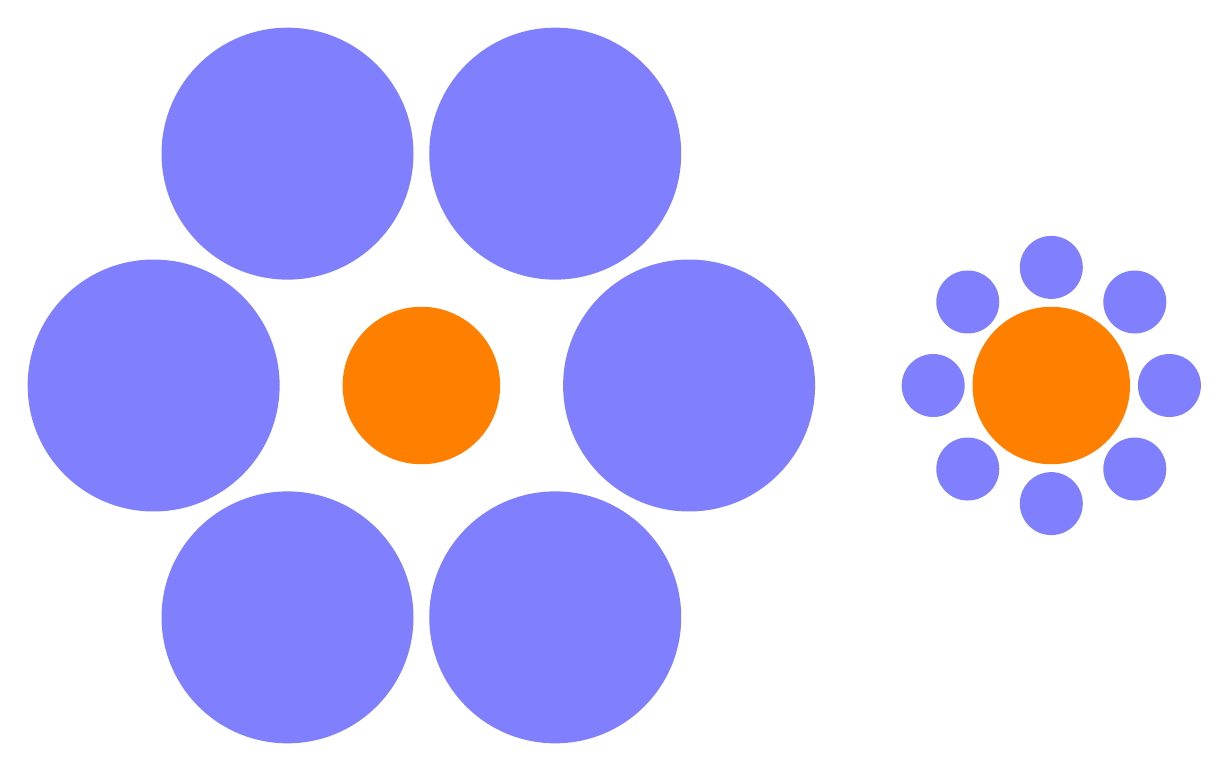
\begin{tikzpicture}
		\def\a{1}   % bán kính 2 hình tròn ở giữa
		\def\b{1.6} % bán kính 6 hình tròn to
		\def\c{.4}  % bán kính 8 hình tròn nhỏ
		\fill[orange] (0,0) circle(\a);
		\foreach \i in {0,60,...,300}
		\fill[blue!50!white]  (\i:3.4) circle (\b);
		\begin{scope}[shift={(8,0)}]
			\fill[orange] (0,0) circle(\a);
			\foreach \i in {0,45,...,315}
			\fill[blue!50!white]  (\i:1.5) circle (\c);
		\end{scope}
	\end{tikzpicture}
	
\begin{tikzpicture}
		\def\a{1}   % bán kính 2 hình tròn ở giữa
		\def\b{1.6} % bán kính 6 hình tròn to
		\def\c{.4}  % bán kính 8 hình tròn nhỏ
		\fill[magenta] (0,0) circle(\a);
		\foreach \i in {0,60,...,300}
		\fill[gray!50]  (\i:3.4) circle (\b);
		\begin{scope}[shift={(8,0)}]
			\fill[magenta] (0,0) circle(\a);
			\foreach \i in {0,45,...,315}
			\fill[gray!50]  (\i:1.5) circle (\c);
		\end{scope}
	\end{tikzpicture}
\end{document}